\section{Evaluation}
\label{sec:evaluation}

The evaluation consists of four parts:

\begin{itemize}
\item Application profiles (\autoref{fig:all-profiles})
\item Online Profiling (\autoref{fig:online-profiling-comparison},
  \autoref{fig:parallel}, \autoref{fig:trigger})
\item Runtime Adaptation (\autoref{fig:all-runtime})
\item Multi-task Scheduling (\autoref{fig:multitask})
\end{itemize}

\subsection{Application Profiles}
\label{sec:application-profiles}

\begin{figure*}
  \centering
  \begin{subfigure}[t]{0.33\textwidth}
    \centering
    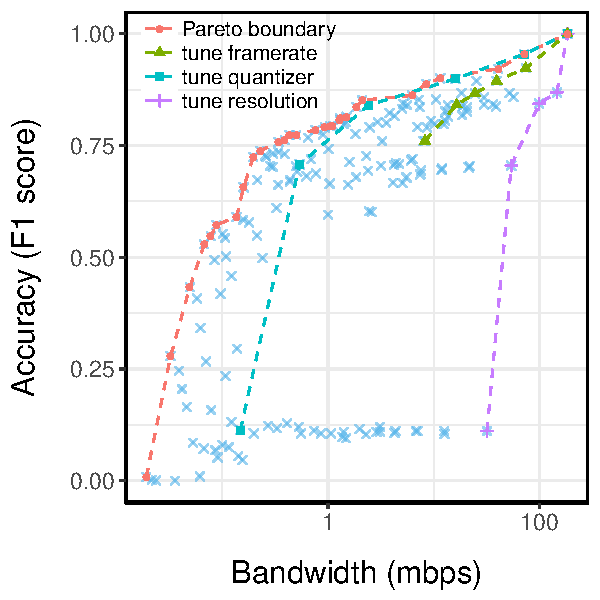
\includegraphics[width=\textwidth]{figures/ped-profile.pdf}
    \caption{Pedestrian Detection}
    \label{fig:pd-profile}
  \end{subfigure}
  ~
  \begin{subfigure}[t]{0.33\textwidth}
    \centering
    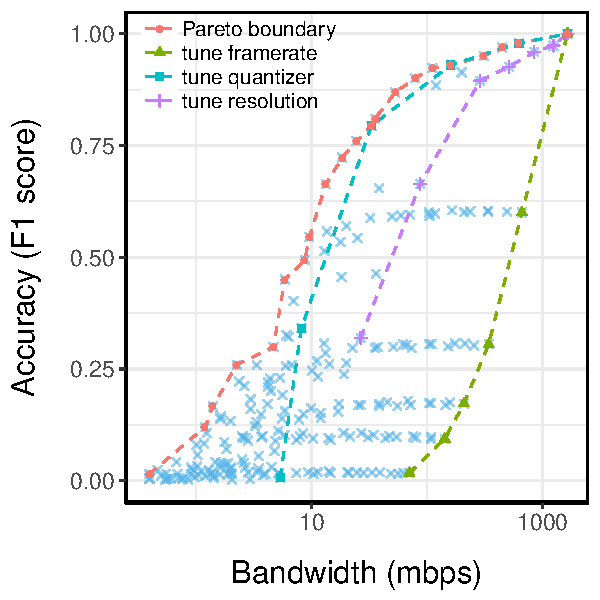
\includegraphics[width=\textwidth]{figures/darknet-profile.pdf}
    \caption{Augmented Reality}
    \label{fig:ar-profile}
  \end{subfigure}
  ~
  \begin{subfigure}[t]{0.33\textwidth}
    \centering
    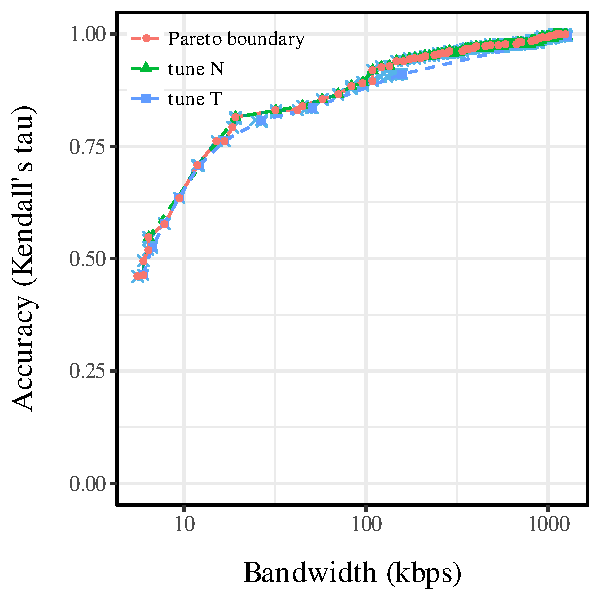
\includegraphics[width=\textwidth]{figures/topk-profile.pdf}
    \caption{Top-k}
    \label{fig:tk-profile}
  \end{subfigure}
  \caption{Application profiles.}
  \label{fig:all-profiles}
\end{figure*}

\subsection{Online Profiling}
\label{sec:online-profiling}

The main challenge with online profiling is the combinatorial space and
efficiency of profiling.

First we validate the demand for online
profiling. \autoref{fig:online-profiling-comparison} shows the difference for
with and without online profiling. Without online profiling, the initial profile
fails to offer optimal degradation soon afterwards.

\begin{figure}
  \centering
  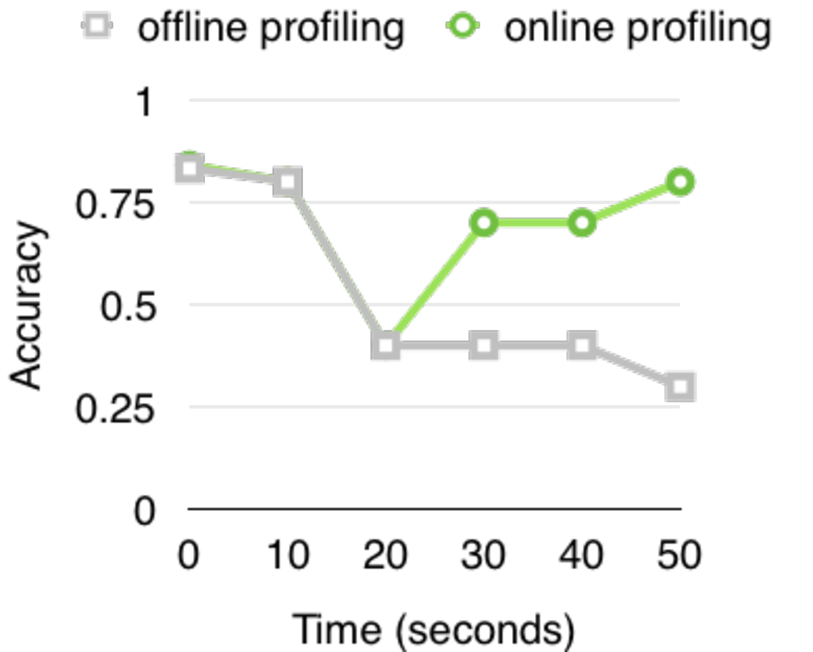
\includegraphics[width=\columnwidth]{figures/offline-online-profiling.pdf}
  \caption{The case for online profiling}
  \label{fig:online-profiling-comparison}
\end{figure}

Naively running profiling online is computational expensive. We evaluate two
solutions regarding the efficiency:

\para{Degradation-aware parallel profiling:} Compare strategies for profiling.
\autoref{fig:parallel} shows our profiling scheduling in comparison with a naive
scheduler.

\begin{figure}
  \centering
  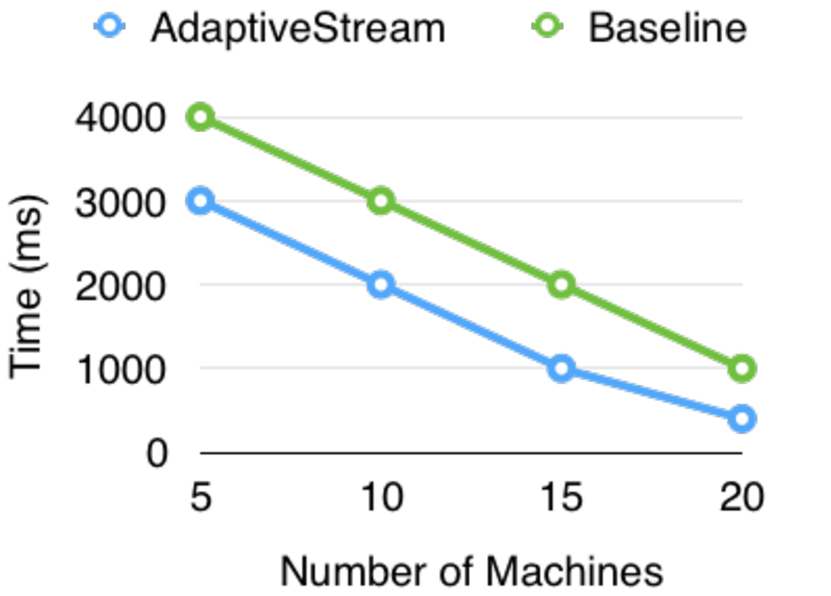
\includegraphics[width=\columnwidth]{figures/parallel-placeholder.pdf}
  \caption{Degradation-aware parallel scheduling}
  \label{fig:parallel}
\end{figure}

\para{Trigger-based profiling:} Only start the profiling when there is
substantial difference. \autoref{fig:trigger-profiling} shows the savings in
trigger-based profiling.

\begin{figure}
  \centering
  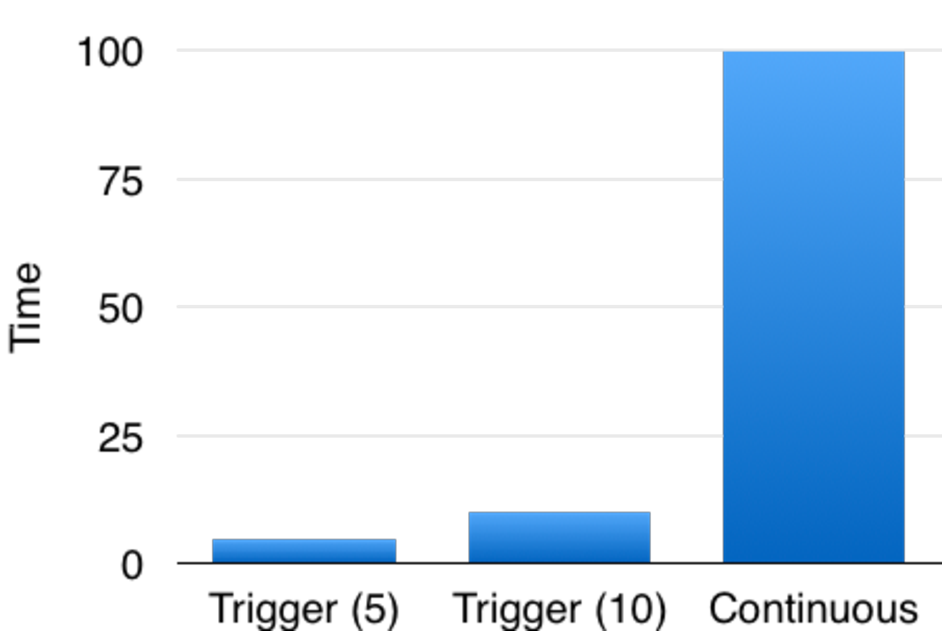
\includegraphics[width=\columnwidth]{figures/trigger.pdf}
  \caption{Trigger-based profiling}
  \label{fig:trigger}
\end{figure}

\subsection{Runtime Adaptation}
\label{sec:runtime-adaptation}

\begin{figure*}
  \centering
  \begin{subfigure}[t]{0.33\textwidth}
    \centering
    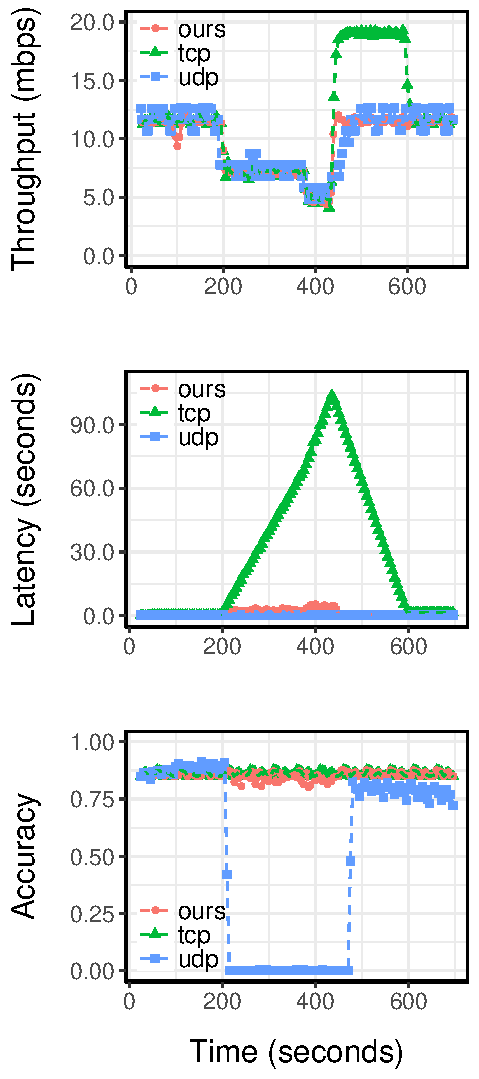
\includegraphics[width=\textwidth]{figures/ped-runtime-verticle.pdf}
    \caption{Pedestrian Detection}
    \label{fig:pd-runtime}
  \end{subfigure}
  ~
  \begin{subfigure}[t]{0.33\textwidth}
    \centering
    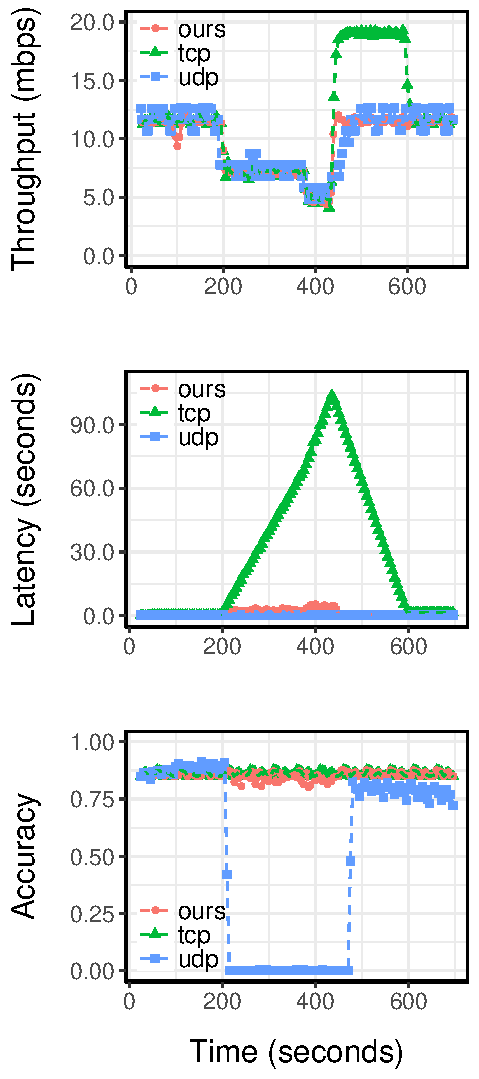
\includegraphics[width=\textwidth]{figures/ped-runtime-verticle.pdf}
    \caption{Augmented Reality}
    \label{fig:ar-runtime}
  \end{subfigure}
  ~
  \begin{subfigure}[t]{0.33\textwidth}
    \centering
    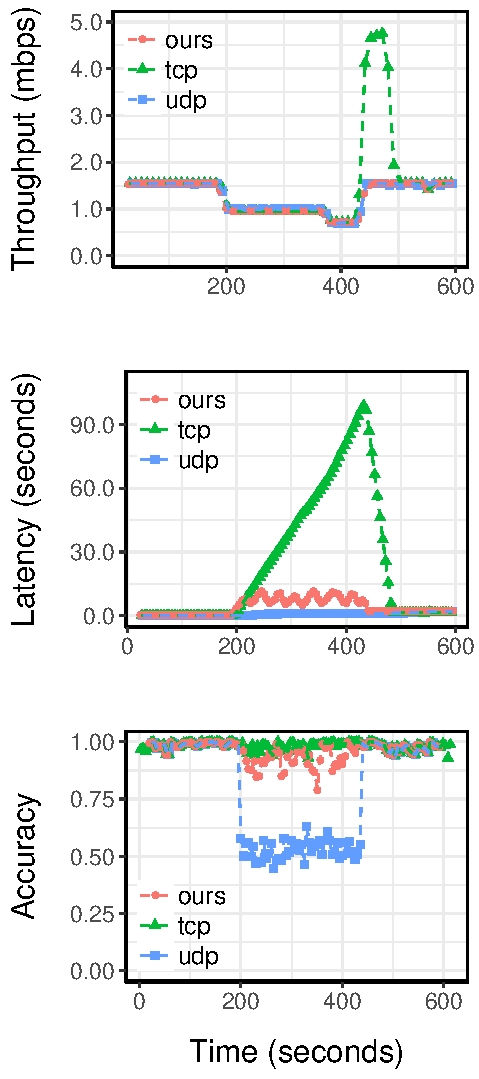
\includegraphics[width=\textwidth]{figures/topk-runtime-verticle.pdf}
    \caption{Top-k}
    \label{fig:tk-runtime}
  \end{subfigure}
  \caption{Application profiles.}
  \label{fig:all-runtime}
\end{figure*}

\subsection{Multi-task Scheduling}
\label{sec:multi-task-sched}

\begin{figure}
  \centering
  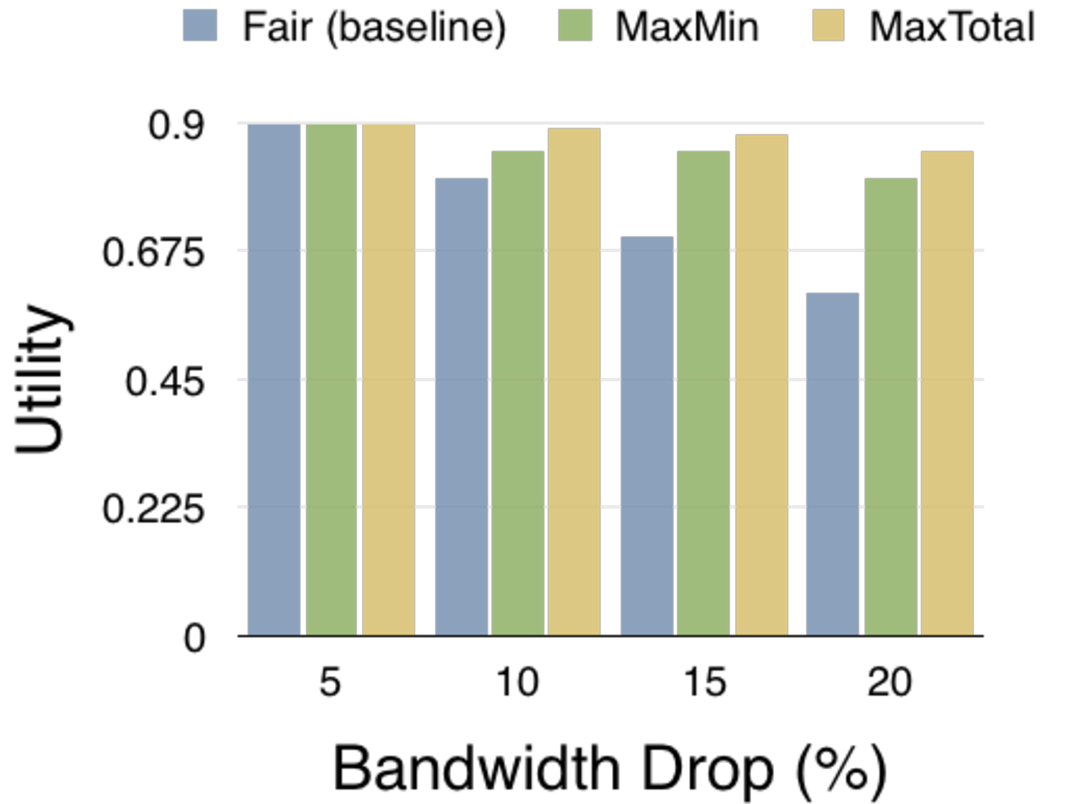
\includegraphics[width=\columnwidth]{figures/multitask.pdf}
  \caption{Multitask Scheduling}
  \label{fig:multitask}
\end{figure}

%%% Local Variables:
%%% mode: latex
%%% TeX-master: "sosp17"
%%% End:
